\documentclass{standalone}
\usepackage{tikz}
\usetikzlibrary{decorations.pathmorphing} % For wavy lines

\begin{document}

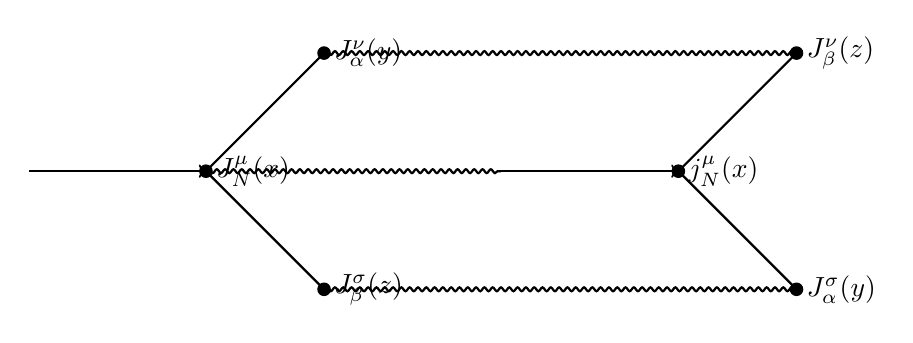
\begin{tikzpicture}[scale=1.5]

% Left diagram
\draw[thick,->] (0,0) -- (1.5,0) node[right] {$J^{\mu}_N(x)$};
\draw[thick,-] (1.5,0) -- (2.5,1) node[right] {$J^{\nu}_{\alpha}(y)$};
\draw[thick,-] (1.5,0) -- (2.5,-1) node[right] {$J^{\sigma}_{\beta}(z)$};

% Right diagram
\draw[thick,->] (4,0) -- (5.5,0) node[right] {$j^{\mu}_N(x)$};
\draw[thick,-] (5.5,0) -- (6.5,1) node[right] {$J^{\nu}_{\beta}(z)$};
\draw[thick,-] (5.5,0) -- (6.5,-1) node[right] {$J^{\sigma}_{\alpha}(y)$};

% Wavy lines (dark gluon exchange)
\draw[decorate, decoration={snake, segment length=3pt, amplitude=.7pt}, thick] (1.5,0) -- (4,0);
\draw[decorate, decoration={snake, segment length=3pt, amplitude=.7pt}, thick] (2.5,1) -- (6.5,1);
\draw[decorate, decoration={snake, segment length=3pt, amplitude=.7pt}, thick] (2.5,-1) -- (6.5,-1);

% Triangles (fermion loops)
\filldraw[black] (1.5,0) circle (1.5pt);
\filldraw[black] (2.5,1) circle (1.5pt);
\filldraw[black] (2.5,-1) circle (1.5pt);
\filldraw[black] (5.5,0) circle (1.5pt);
\filldraw[black] (6.5,1) circle (1.5pt);
\filldraw[black] (6.5,-1) circle (1.5pt);

\end{tikzpicture}

\end{document}